\documentclass[tikz]{standalone}

\begin{document}

\bfseries 
\footnotesize 
\begin{tikzpicture}[line width=0.8mm,scale=1.3]

	% === REFFERENCES === (((
	\node [opacity=0.7] at (0,0) 
	{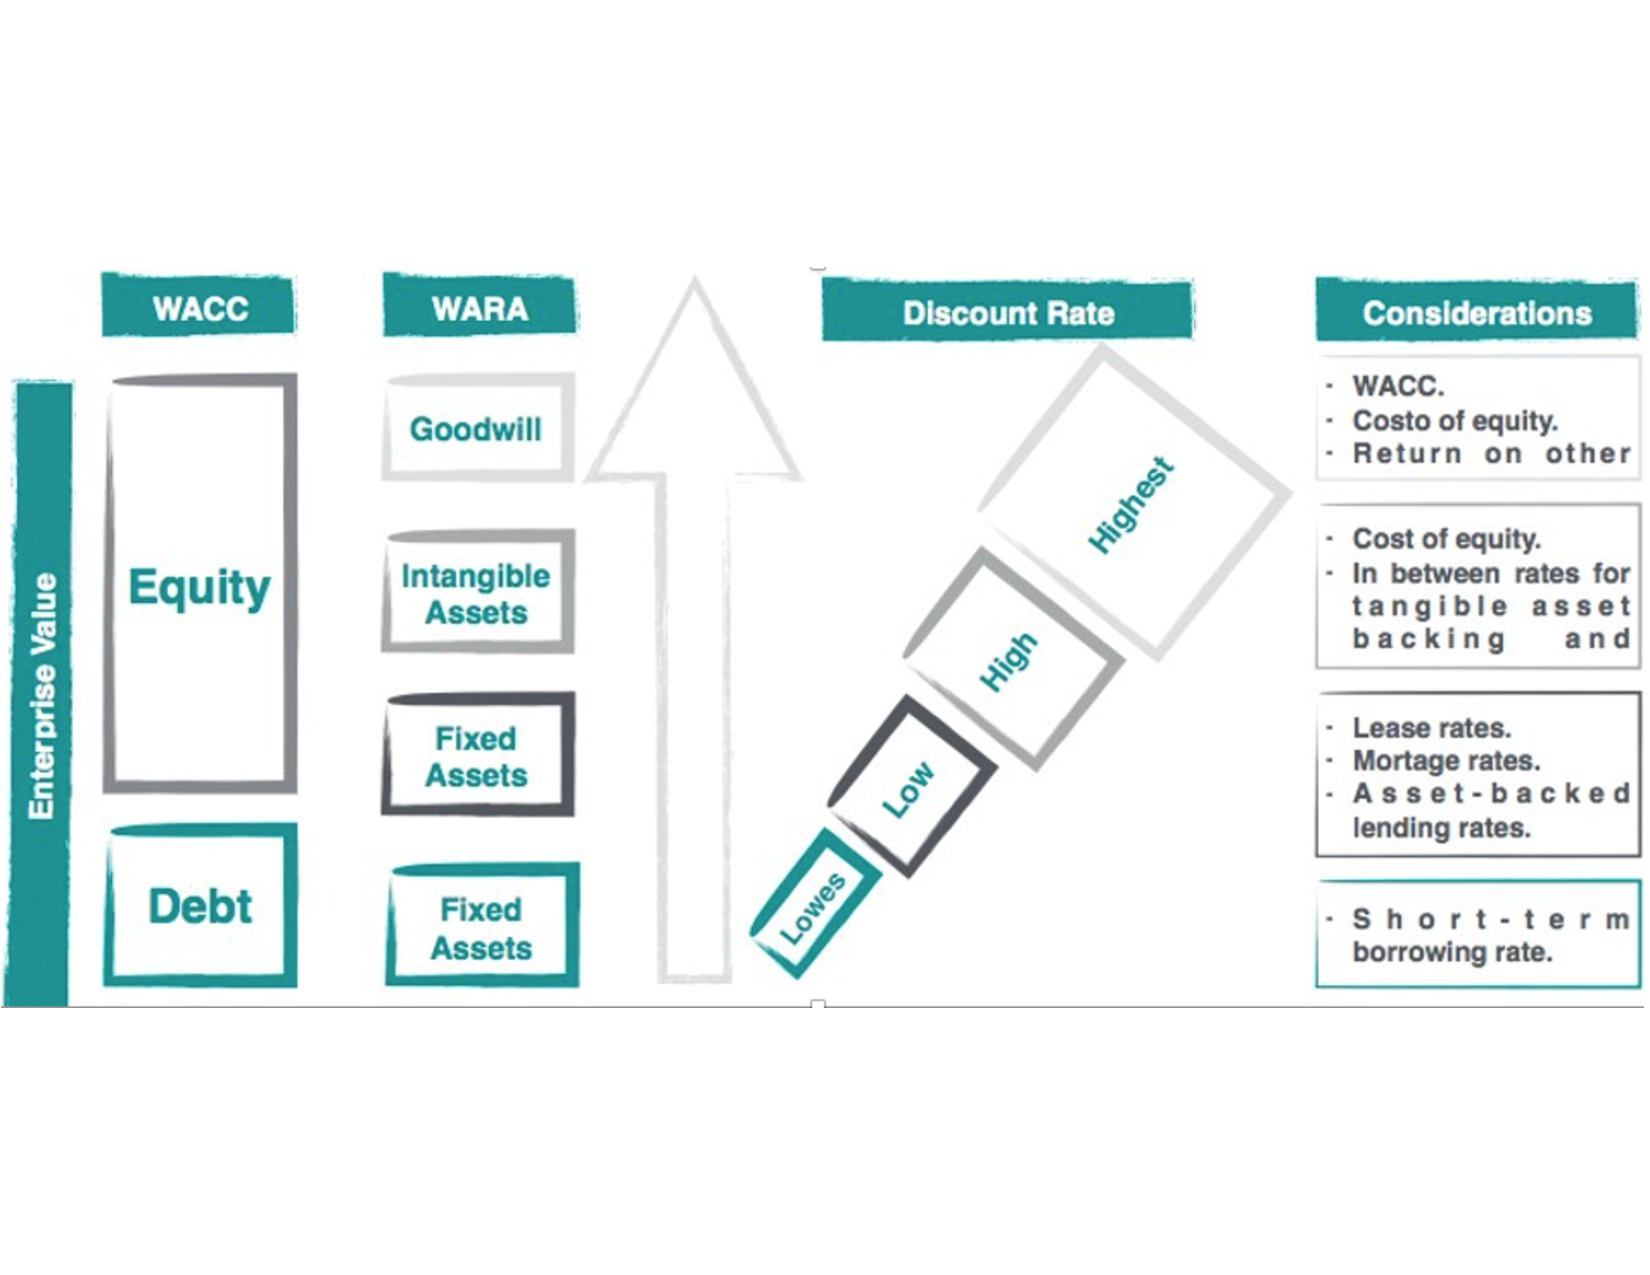
\includegraphics[width=  13cm, page = 1]{image}};
	\draw [help lines] (-5,-2.5) grid (5,2.5);
	\fill [red] (0,0) circle (2pt);
	% )))

	\draw [gray] (-4.4,-0.9) rectangle node [text=teal] 
	{\large Capital} ++(1.3,2.5);
	\fill [teal] (-4.9,-2.3) rectangle 
	node [rotate=90,text=white] {Valor Emmpresarial} ++(0.3,4);
	\draw [teal] (-4.4,-2.1) rectangle node {Deuda} ++(1.3,1);


\end{tikzpicture}

\end{document}
